In the domain of drone systems, effective communication stands as a central pillar for operational success.
Communication with drones refers to the process of transmitting and receiving information between a drone and a remote control device or computer system. 
It involves the use of various technologies, including Wi-Fi, Bluetooth, and cellular, to control the drone and receive real-time data and feedback.

One of the most essential features of an ideal communication infrastructure for drone applications is the possibility of handling all the data in real-time settings.
In other words, it must guarantee a low-latency and reliable channel of communication.

Having an efficient communication channel is only a part of the success of the communication infrastructure. 
To provide a robust and efficient communication infrastructure, we need an organized structure for routing the data specifically to the target component in charge of processing the information.

The last important characteristic of an ideal communication infrastructure is having a simple and intuitive interface.
This feature is of primary interest in our programming environment because it allows beginners to use it without effort.

This chapter focuses on a crucial element of our drone programming environment: the Communication Framework. 
Its purpose is to handle all the communication between the ground station and the flying drone, providing all the characteristics of the ideal communication infrastructure.

More in detail, the Communication Framework is a software component hosted on the ground station 
that allows the user to establish effective communication between the script running on the ground station and the drone.

The Communication Framework manages the communication stream into two separate flows: parameter setting and telemetry logging.
The former is the flow of communication that is directed from the ground station to the drone; it is used to set configuration parameters onboard the drone.
The latter is the opposite flow of communication, from the drone to the ground station, and it is used to receive the telemetry data of the drone, allowing for better control.


\section{The Communication Infrastructure}\label{sec:communication_infrastructure}
Before diving into the details of our Communication Framework, it is crucial to understand the underlying communication infrastructure of the native Crazyflie platform.

As described in Section~\ref{sec:ecosystem_oveerview}, our programming environment is spread into two main devices: the ground station and the drone.
The drone's firmware is written in C++ and runs on a small board with limited resources. On the other side, the ground station runs Python scripts
that control the drone's behavior. The heterogeneity between these two subsystems increases the complexity of the communication process.

The platform uses a custom network protocol called CRTP to overcome all these challenges. 
CRTP was designed to allow packet prioritization to help real-time control of the Crazyflie; in the current implementation, the link guarantees strict packet ordering.

As shown in Figure~\ref{fig:communication_stack}, the Crazyflie communication is implemented as a stack of independent layers.
Every layer of the communication stack has two parallel implementations, one hosted in the firmware onboard and the other on the ground station's software.

\begin{figure}[tb]
    \centering
    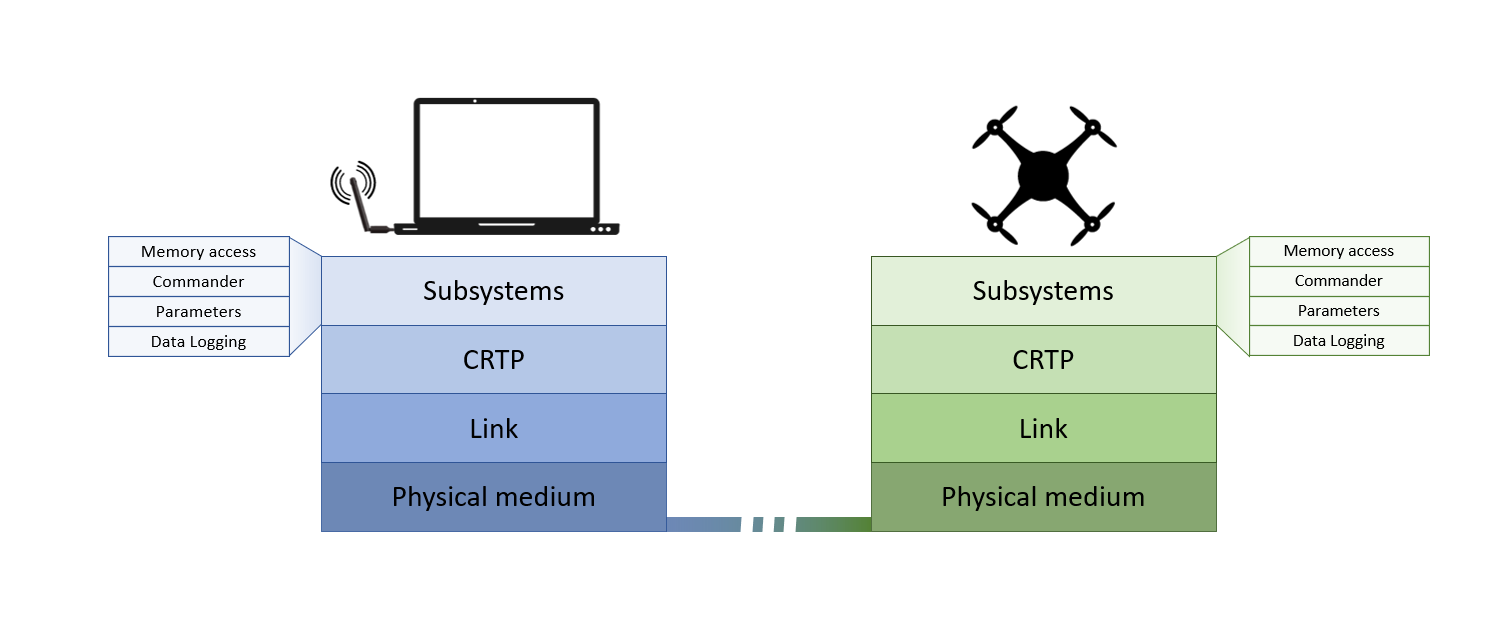
\includegraphics[width=0.9\textwidth]{communication/communication_stack}
    \caption[The Crazyflie communication stack]{The Crazyflie communication stack is composed of 4 independent layers: Subsystems, CRTP, Link, Physical medium}
    \label{fig:communication_stack}
\end{figure}

The physical layer is responsible for transmitting packets to and from the Crazyflie. 

The link layer implements safe and ordered packet channels to and from the Crazyflie. This layer abstracts the physical medium and implements one transmitting and receiving packet channel to and from the Crazyflie.

The CRTP layer introduces the concept of a logical packet; each packet measures 32 Bytes and is composed of three parts: port, channel, and payload.
The tuple \textit{port:channel} allows the packet to be delivered to the specialized subsystem that receives and processes the message.

The Subsystem layer is the final part of the communication process. It represents the part of the system (Crazyflie firmware or ground station software) that elaborates the information.
In the higher-order layer, we can identify four principal subsystems:
\begin{itemize}
    \item \textbf{Memory access} -- that manages memory operation on the Crazyflie's physical memories, e.g., trajectory uploading.
    \item \textbf{Commander} -- that send/receive control set-points.
    \item \textbf{Parameters} -- that manages read/write operations on configuration parameters of the Crazyflie.
    \item \textbf{Data Logging} -- that handles logs of telemetry data sent periodically from the Crazyflie to the ground station. 
\end{itemize} 

The first two subsystems (memory access and commander) are the simplest, with a straightforward implementation. 
They expose some methods through an API, and when called, they craft a packet, fill it with parameters data, and send it to the link layer.
On the other side, the same subsystem receives the packet, unpacks the data, and executes the desired function.

Conversely, the parameters and data logging subsystems have some peculiarities that make them more complex. 
In particular, the parameters subsystem allows performing read/write operations with acknowledgments of the successful operation.
The data logging subsystem, instead, must support periodical updates of telemetry data.
Moreover, both subsystems must handle a variety of variables with different types.

The communication infrastructure of the Crazyflie platform guarantees an efficient communication channel with a structured routing mechanism over the custom protocol CRTP.
This basic infrastructure allows a developer to communicate with Crazyflie at a very low level.
The problem is the absence of an accessible interface; the developer must profoundly understand the underlying structure and communication mechanism to use it.

The Communication Framework that we designed and developed is meant to wrap basic infrastructure to offer the developer an easier and more accessible communication interface.
Moreover, we managed all the low-level control mechanisms automatically. 
In this way, the developer does not need to worry about low-level operation but still preserves performance.

In particular, we decided to simplify the interface of the two complex subsystems and offer the user a more usable and efficient way to handle data logging and parameters.

\section{Design}\label{sec:communication_frameworks_design}

The Communication Framework is a software component that provides an easy and accessible way to set parameters onboard the Crazyflie and to log telemetry data.
This component is part of the ground station's software and has been designed as a publish/subscribe system.

Every CRTP data that is routed to the parameter or logging subsystem is managed by the Communication Framework and stored in a central repository.
Every other software component or script interested in such data can use the Communication Framework to access the repository and subscribe for value updates.

Given the profound semantic difference between the logging and parameters subsystems, we decided to keep the two concepts separated inside the Communication Framework.
For this reason, we developed two different Communication Managers, one for every subsystem. The two implementations, namely the Logging and the Parameters Manager, 
shares the publish/subscribe design structure, but they slightly differ in the management of the updates in the repository.

\subsection{The Logging Manager}\label{subsec:logging_manager}

As described above, the Logging Manager is one of the two implementations of the Communication Framework. 
In particular, the role of the Logging Manager is to handle the setup and the periodic updates of telemetry data sent from the Crazyflie.

Given the asynchronous nature of telemetry data, we designed the Logging Manager as a publish/subscribe system.

In particular, the internal structure of this component is composed of two main parts: a values repository to store telemetry data and a notification system.

The value repository is used to hold on the ground station the telemetry data sent by the Crazyflie.
It is implemented with a dictionary of key-value pairs to guarantee immediate access to the information held.
More in detail, each variable, identified by a unique key, represents an entry inside the values repository; the value of the entry is the last updated value of the logged variable.

The second part of the Logging Manager is the notification system that follows the publish/subscribe design pattern.
The publish/subscribe design pattern establishes a communication model where components (subscribers) express interest in specific events or messages, and other components (publishers) broadcast relevant information to all interested subscribers.

To implement such a pattern, the notification system inside the Logging Managers stores the reference of subscribers interested in the variables updates in a separate repository.
Each reference consists of a predicate function to allow filtering updates and a callback function to effectively notify the subscriber when the predicate is satisfied with the new value.

To better understand the working principle behind the Logging Manager, we will present an example of utilizing the Logging Manager, focusing on what occurs behind the scenes.
To guide the understanding of the example, we have illustrated in Figure~\ref{fig:logging_manager} the Logging Manager's workflow.

Let us consider a developer implementing a drone application to navigate the drone through an obstacle course using EasyFly.
To implement its solution, they will surely need to use the estimated position in the environment. 
To do so, after creating the main ECF component, they can use the Logging Manager to request the desired telemetry data.
In particular, they will request three state variables: \( position_x \), \( position_y \), and \( position_y \).

Upon receiving this request, the Logging Manager will prepare a log configuration and send it to the Crazyflie.
When the Crazyflie receives the log configuration, it can send telemetry data at periodic intervals.
Every time new data is available, the Logging Manager can store it inside its values repository.

The simple request for position data does not automatically activate the notification system.
The developer must subscribe to the notification system to receive notifications when the values are updated.
To do so, they can define a callback function and, optionally, a predicate function that filters only the valuable notification.

Suppose the developer needs to add other telemetry data, for example, the Multiranger front sensor readings \( range_front \). 
In that case, the Logging Manager will optimize the number of logging configurations used, allowing for the best possible log performance.

\begin{figure}[tb]
    \centering
    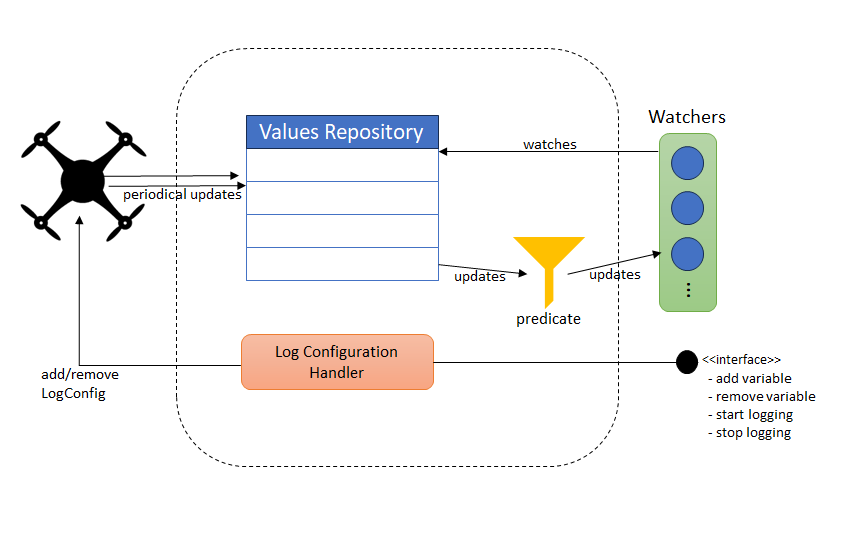
\includegraphics[width=0.9\textwidth]{communication/logging_manager}
    \caption{Logging Manager's workflows.}\label{fig:logging_manager}
\end{figure}

\pagebreak% REASON FORMAT 

\subsection{The Parameters Manager}\label{subsec:parameter_manager}

The other implementation of the Communication Framework, the Parameters Manager, manages the configuration operations of the Crazyflie.
The Crazyflie 2.1 allows the users to set parameter values to configure the desired setup. 
An example of a parameter could be the selected state estimator, i.e., Extended Kalman Filter or Complementary Filter (See Section~\ref{sec:state_estimate_and_control}).

Following the same structure as the Logging Manager, also the Parameters Manager has one value and one subscriber repository where it stores, respectively, the current value for tracked parameters and the references of subscrbers for each variable.

Conversely, variable updates are managed slightly differently with respect to the Logging Manager. 
In fact, the underlying parameters subsystem does not have a periodic update of values; instead, the updates happen only when the parameter's value is effectively changed onboard.
In other words, the Parameters Manager only receives and processes an update when the Crazyflie acknowledges a state change in the parameter's value.
 
Figure~\ref{fig:parameters_manager} represents the operations workflow inside the Parameters Manager. When needed, usually before the takeoff,
the script can use the Parameters Manager to read or write configuration values. 

Read and write operations are processed straightforwardly with a request-response messages exchange.
For read operations, the request contains the variable's name, and the Crazyflie's response contains the current value of the requested parameter.
For write operations, the request contains the variable's name and the new value, and the Crazyflie's response includes the newly updated value. 
The response is usually used to acknowledges the success of the write operation.

As for the Logging Manager, once the Parameters Manager receives a value from the Crazyflie, the internal notification system is used to notify subscribers.

\begin{figure}[tb]
    \centering
    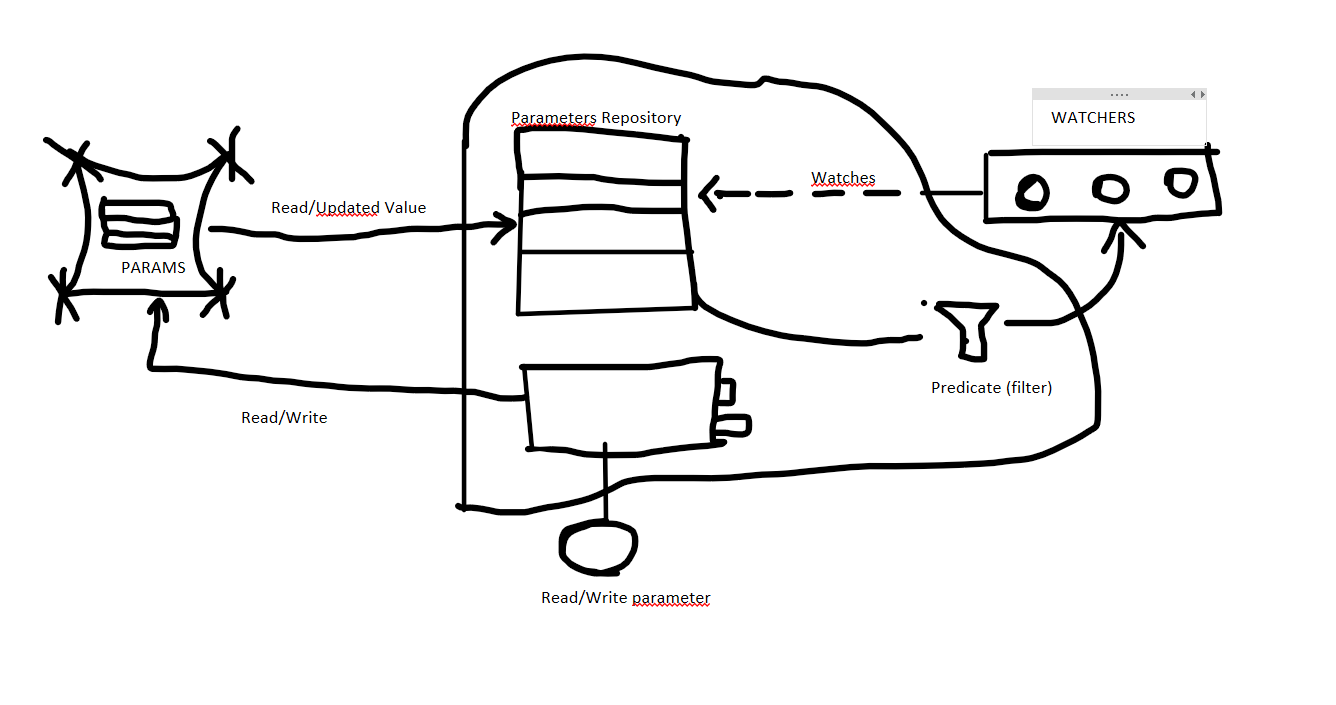
\includegraphics[width=0.9\textwidth]{communication/parameters_manager}
    \caption{Parameters Manager's workflows.}\label{fig:parameters_manager}
\end{figure}

